
\section{Solução de Eletrônica}

\subsection{Central}

Dentro do sistema, a central servirá como receptora de todos os dados emitidos pelo tanques, por processar dados e enviá-los para um servidor web através de seu módulo Wi-Fi , e como servidor e central de comando para os administradores do sistema.

O hardware da central será bastante minimalista, sendo composto, no total, por uma placa Raspberry Pi 3, cartão microSD, módulo nRF24L01+ com antena e fonte de tensão, onde tudo estará acondicionado em um gabinete adaptado para os componentes.

A placa Raspberry Pi 3 foi adotada como a plataforma da central por vários motivos, que são: serve como sistema computacional capaz de rodar o sistema operacional linux e acomodar um pequeno servidor web, ser mais barato e ter menor consumo elétrico que um computador desktop convencional, possuir pinos com função de IOs similar aos microcontroladores, unificando a função de servidor com a de microcontrolador, e por possuir, assim como a plataforma Arduino, bibliotecas de rede de alto nível para o módulo de rádio RF24, possibilitando funções poderosas de comunicação entre cada módulo que serão explicadas mais adiante, na seção específica sobre comunicação.

Assim, será possibilitado que a central esteja conectada com outros computadores e dispositivos internos por meio de uma rede wi-fi e também poderá se comunicar a longa distância com todos os alimentadores pelo módulo de rádio RF24.

\begin{figure}[!h]
\centering 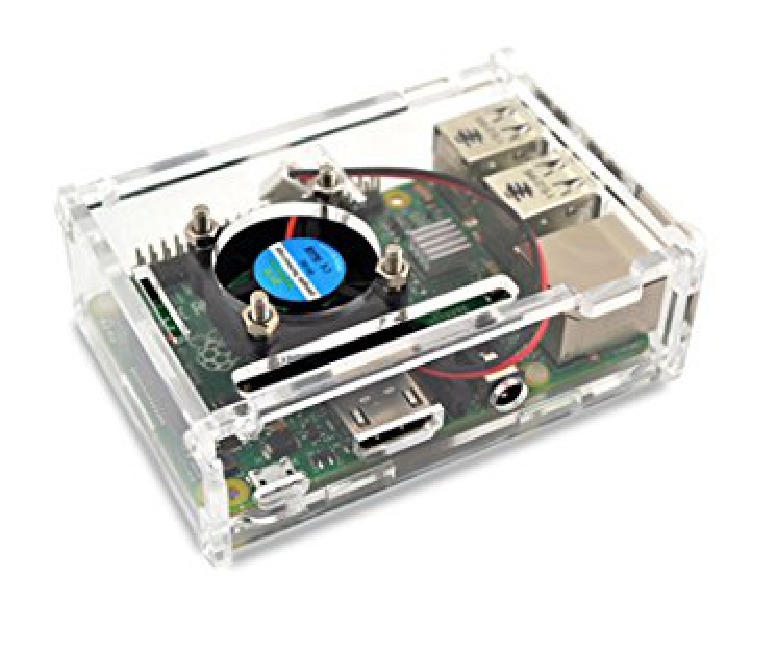
\includegraphics[scale=0.5]{raspberry_case}
\caption{Ilustração do dispositivo central montado}
\label{rasp}
\end{figure}

O sistema rodará a partir de dois processos,  sendo executados de forma paralela, em que um é o processo responsável pelo controle da comunicação entre os módulos e envio de dados, desenvolvido integralmente em linguagem C++ para linux, e o outro é o processo responsável pelo servidor e central de comando do usuário.

O processo responsável pela comunicação entre os módulos funciona, basicamente, a partir de 3 rotinas, que são: RX, TX e Sinc. A descrição de cada rotina é o seguinte:

    \begin{itemize}
\item{RX: Recebe os dados lidos dos alimentadores de cada tanque. Todos os dados recebidos são organizados para serem registrados no banco de dados do servidor.}
\item{TX: Envia o horário atual e as diretrizes de funcionamento para cada alimentador}
\item{Sinc: Sincroniza  com o processo do servidor todas as configurações a serem definidas nos alimentadores e todos os dados recebidos dos alimentadores.}
\end{itemize}


\subsection{Tanques}

O componente principal do sistema embarcado nos tanques é o microcontrolador ATmega328p, sua escolha deve-se ao fato da biblioteca utilizada para aplicar o protocolo de rede em malha para comunicação entre os módulos nRF24L01+ (explicados mais adiante) ser projetada para aplicação em Raspberry pi e microprocessadores da família ATmega.
O ATmega328p é um microcontrolador de 32 registradores de propósito geral e possui uma memória Flash de 32Kbytes programável, ele possui 23 pinos de propósito geral, sendo que 6 podem também ser utilizados como entrada anlógica. Ele possibilita comunicação do tipo SPI (Serial Peripheral Interface), esta comunicação foi utilizada no projeto para fazer a comunicação com os módulos nRF24L01+. Este microcontrolador também permite comunicação do tipo $I^{2}C$, comunicação serial síncrono utilizada no projeto para conectar a placa principal do tanque com a placa dos sensores \cite{atmel:atmega328p}. A figura abaixo mostra este microcontrolador:

\begin{figure}[!h]
\centering 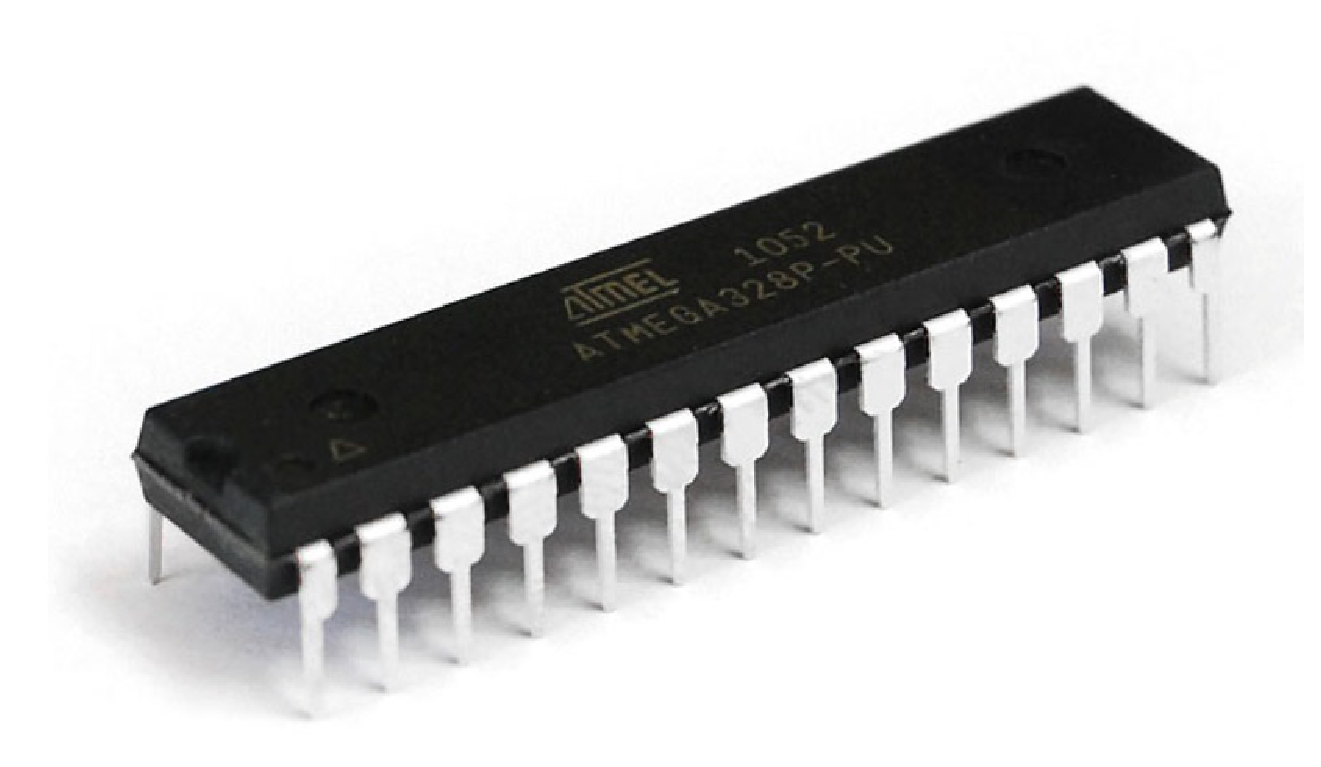
\includegraphics[scale=0.3]{atmega}
\caption{ATmega328p.}
\label{atmega}
 \end{figure}

 Um dos pontos críticos do projeto é a alimentação dos peixes no horário correto, uma das opções seria utilizar a temporização interna do ATmega mas o seu problema é que ela é zerada quando o microcontrolador é desligado. Foi necessário então procurar uma solução mais confiável, a solução escolhida foi utilizar o CI DS1307 que é alimentado por uma bateria própria. Ele é um relógio/calendário BCD que transfere dados via $I^{2}C$, ele provê informações de segundo, minuto, hora, dia, semana e ano. Ele pode ser programado, no projeto esta funcionalidade é utilizada para que ele sincronize seu horário.

Para evitar a desligamento do sistema devido a descarga da bateria e a consequente interrupção da alimentação dos peixes, é necessário realizar o monitoramento do nível da bateria que alimenta o sistema. O monitoramento é feito por uma porta analógica, ele leva em conta duas características importantes da bateria: nível máximo quando estiver carregada, sendo considerado como 100\%, e o nível mínimo que ela pode chegar sem ser danificada, sendo considerado 0\%. Caso o valor da bateria seja maior do que o valor máximo de entrada da porta analógica então deve ser feito um circuito divisor de tensão, de acordo com a figura abaixo:
A equação \ref{divTensao} é usada para verificar quais serão os resistores que devem ser usados para construir o divisor.

\begin{figure}[!h]
\centering 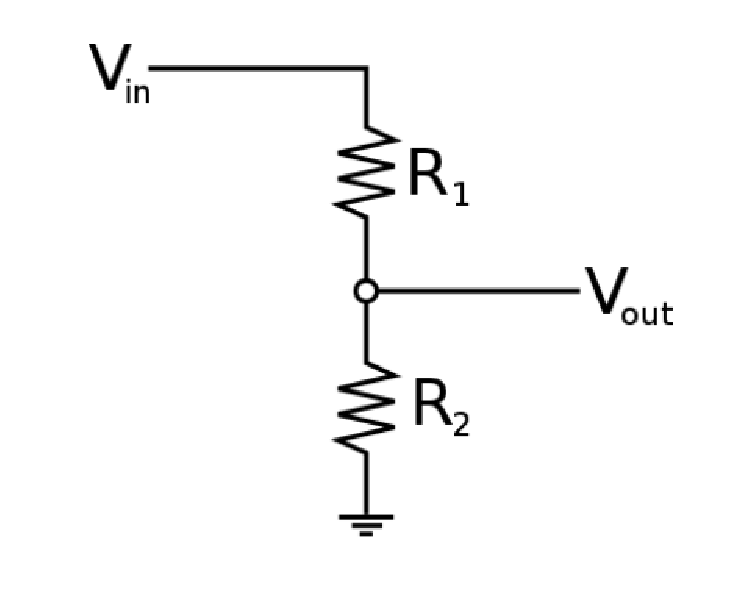
\includegraphics[scale=0.3]{divisor_de_tensao}
\caption{Divisor de Tensão}
\label{divisortensao}
 \end{figure}

\begin{equation}
\label{divTensao}
	V_{out}=V_{in}\frac{R_{2}}{R_{1}+R{2}}
\end{equation}

Onde $V_{in}$ é o nível máximo de tensão da bateria e $V_{out}$ o nível máximo que pode ser colocado na porta ADC \cite{battery}.  No cálculo dos valores dos resistores foi considerado que a corrente deve ser baixa tanto para garantir o baixo consumo de potência como para não danificar pino de referência do microcontrolador. Considerando $R_{1}=1M\Omega$ para que a corrente seja baixa e esteja na caso dos microamperes, $R_{2}$ pode ser calculado:

\begin{equation}
\label{divTensao2}
V_{out}=V_{in}\frac{R_{1}}{R_{1}+R{2}}\rightarrow (R_{1}+R_{2})3,3=12R_{2}\rightarrow R_{1}=2,636R_{2}\rightarrow R_{2}=380k\Omega
\end{equation}

O regulador de tensão utilizado para estabilizar a tensão da bateria que alimenta o sistema dos tanques utilizados foi o LM2576.
\cite{ti:lm2576}

O sistema do tanque também contém um medidor de nível de ração do reservatório, esta medida é feita com o uso do sensor ultrassônico que indica o nível de ração baseado no valor de distância medido. O sensor utilizado foi o HC-SR04.

\subsection{Sistema de Comunicação}

A comunicação entre os tanques e a base, bem como o sistema em geral são ilustrados pela figura abaixo:

\begin{figure}[!h]
\centering 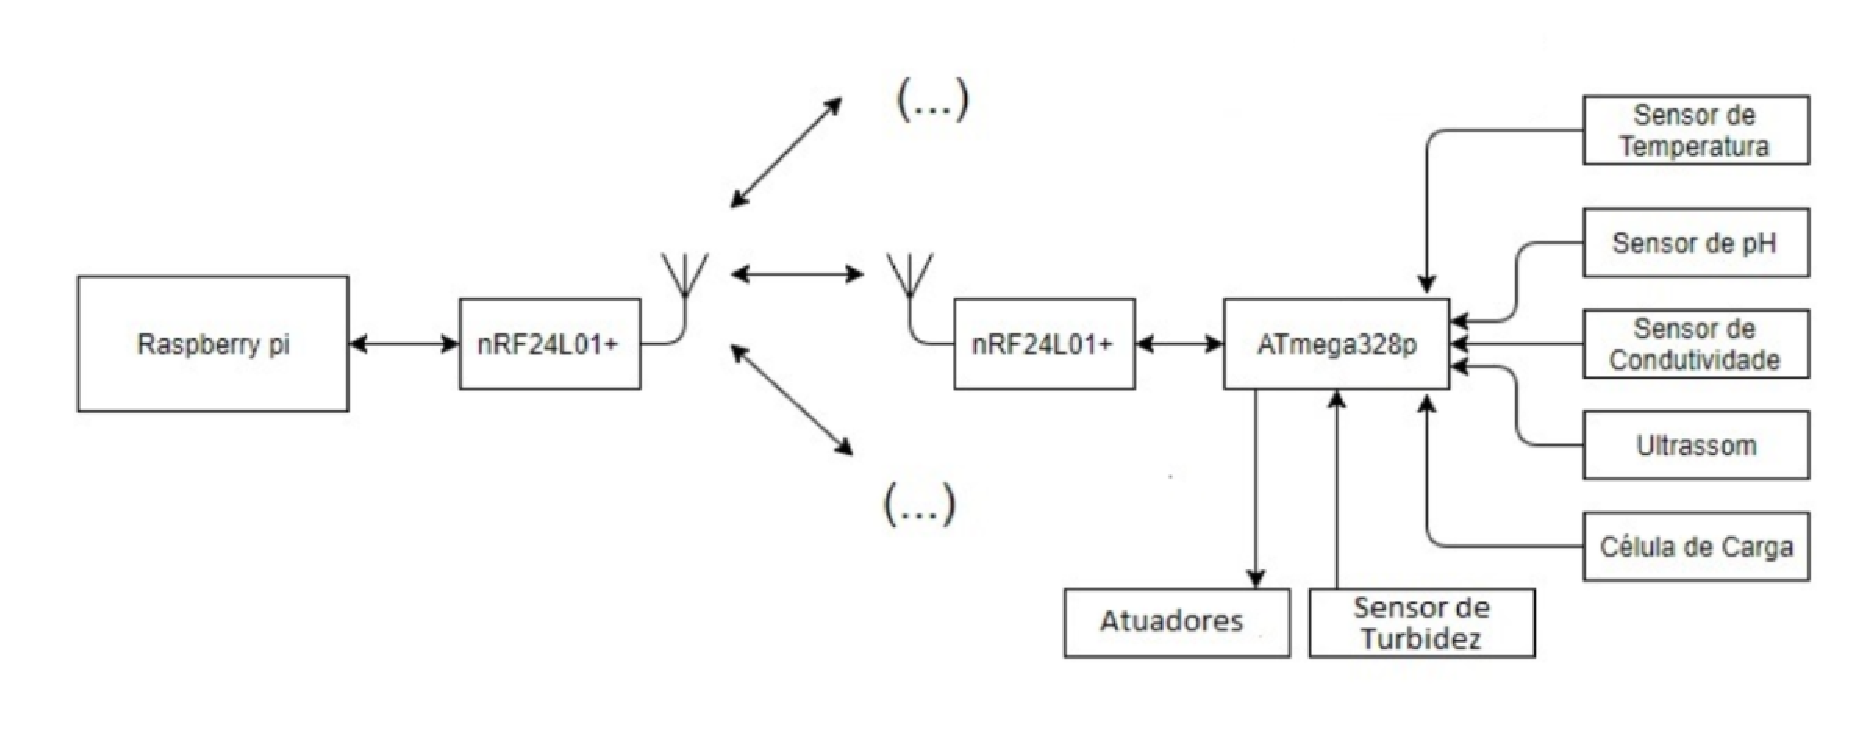
\includegraphics[scale=0.4]{diagrama_de_comunicacao}
\caption{Diagrama de Blocos para o sistema.}
\label{diagramacomunicacao}
 \end{figure}

\pagebreak

Os módulos utilizados para a comunicação entre os dispositivos foi o módulo nRF24L01+, este dispositivo foi escolhido por ter um preço acessível e funcionalidades que suprem as necessidades do projeto. Este módulo contém um chip transceptor de 2,4 GHz para uso em aplicações wireless de baixo consumo de potência, ele é configurado pelo microcontrolador ao qual ele está acoplado através de um protocolo Serial Peripheral Interface (SPI). O transceptor pode ser  configurado através de registradores acessados por SPI. Ele possui uma antena de 2 dBi com um PA de 20 dB.

Realizando testes para verificar se qual a distância máxima que os dados são enviados e recebidos com confiabilidade o grupo obteve o valor de 300 metros, valor suficiente para o projeto que tem como máxima distância entre a central e o tanque mais longe de 200 metros.

Os módulos de comunicação acoplados aos tanques e ao dispositivo central permitem a construção de uma rede para a troca de informações, a topologia de rede escolhida para esta aplicação foi a de rede em malha. A escolha pela topologia em malha foi feita pois ela permite conectar e desconectar tanques além de diminuir os problemas de alcance de dados, devido ao fato dos pacotes poderem passar por diversos dispositivos antes de chegarem a central.

Para a aplicação desta topologia de rede nRF24L01+ existe a biblioteca RF24Mesh projetada para o uso em Raspberry pi e nos microcontroladores ATmega. De acordo com o desenvolvedor da biblioteca, a mesma provê um sistema de endereçamento e roteamento automático dos módulos RF24 permitindo que grandes redes sem fio de sensores sejam construídas. Ela funciona utilizando um nó mestre, que no caso do projeto é a base, este nó mestre rastreia os IDs dos dispositivos que estão na rede, caso um dispositivo seja movido pela rede ela se auto organiza se reconfigurando novamente \cite{meshnetwork}.

O dispositivo dentro da rede pode estar em dois estados em relação à comunicação: escutando ou enviando informações. Ele passa a maior parte do tempo escutando a rede para verificar se chegou algum pacote para ele guardar ou reenviar pela rede, isto é feito através da função network.available() pertencente à biblioteca RF24Network a qual a biblioteca RF24Mesh utiliza em sua construção, quando um pacote é recebido um cabeçalho que vem juntamente com ele é lido para verificar qual o tipo de informação chegou (os tipos de informações trocadas serão apresentadas mais adiante). Este pacote de informação é lido então pela função network.read() onde são guardadas na memória para serem utilizadas posteriormente. Tanto a central quanto os tanques seguem este procedimento para receber as informações, ficam escutando a rede e caso alguma informação endereçada para eles cheguem eles verificam qual o cabeçalho do pacote que chegou, para saberem que tipo de pacote é aquele, e guardam a informação para seu uso posterior.

Quando está no horário de escrever algo (central escrever para algum nó específico ou algum nó escrever para a central) a função mesh.write() é então chamada, os parâmetros colocados dentro desta função são o pacote de informação a ser enviado, o cabeçalho que define o tipo de pacote que está sendo enviado e o nó para qual será enviado (caso seja a central este nó é o nó zero). É necessário também que a conexão seja verificada, para que, caso o dispositivo esteja enviando o pacote e não obtenha resposta, ele se reconfigure dentro da rede mudando seu endereço, estes dois processos são realizados pelas funções mesh.checkConnection() e mesh.renewAddress() respectivamente.

Os pacotes de informações enviados da central para os tanques são dois: um pacote contendo a hora local para que se possa programar o relógio DS1307 sincronizando a rede, e o pacote contendo as informações acerca do horário de alimentação e quantidade de alimento. Já o pacote enviado dos tanques para a central contém informações acerca da bateria e dos sensores daquele tanque em específico. Estes pacotes são structs definidas no início do programa.

Pacote enviado do tanque para a central:

\begin{figure}[!h]
\centering 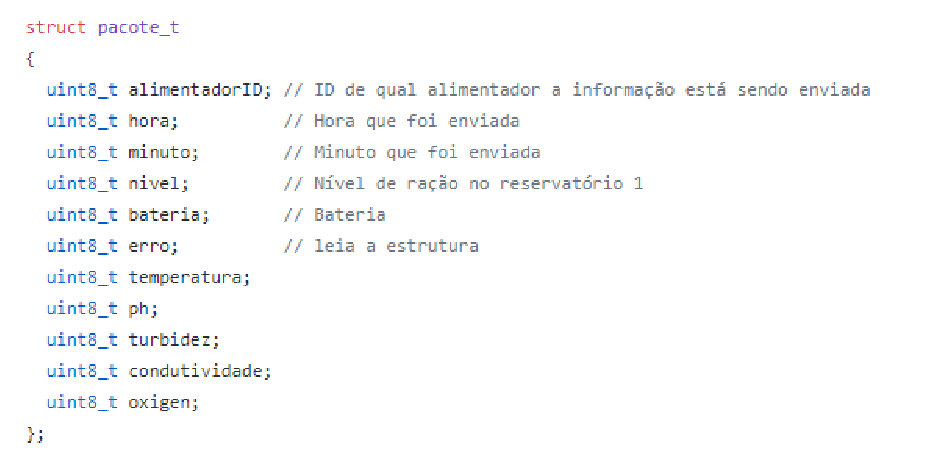
\includegraphics[scale=0.5]{pacote_t}
\label{pacote_t}
\end{figure}

Pacote enviado da central para o tanque contendo informações acerca do horário de alimentação dos peixes:

\begin{figure}[!h]
\centering 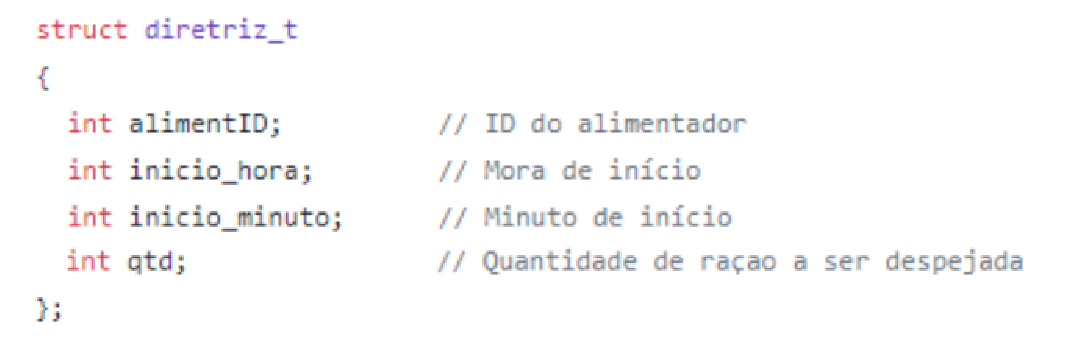
\includegraphics[scale=0.5]{diretriz_t}
\label{diretriz_t}
\end{figure}

Pacote enviado da central para os tanques contendo as informações para a sincronização com o horário da base através da programação do DS1307:

\begin{figure}[!h]
\centering 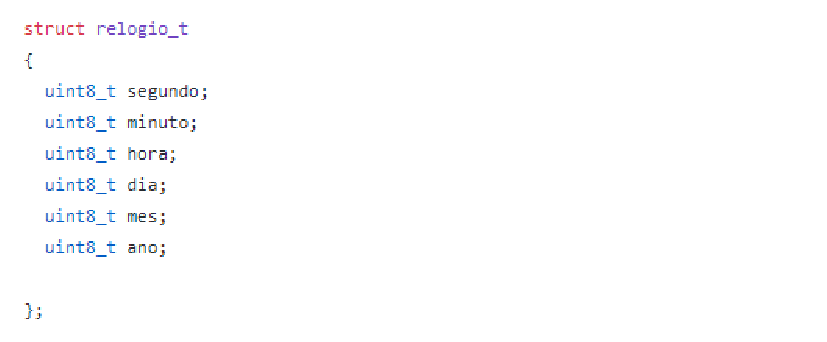
\includegraphics[scale=0.5]{relogio_t}
\label{relogio_t}
\end{figure}

As informações enviadas para os tanques acerca da alimentação devem ser obtidas da aplicação web onde elas são colocadas, para isto um módulo python projetado pela equipe de software foi instalado na raspberry pi. Este módulo gera um arquivo .txt com estas informações que são lidas pelo programa projetado pela equipe de eletrônica e enviadas. As informações recebidas dos tanques pela central também são escritas em um arquivo .txt que é lido pelo módulo em python e enviado para o servidor web onde as informações serão exibidas ao usuário.

\subsection{Sistema de Controle Para a Alimentação}

Para o controle da quantidade de ração despejada foi necessário projetar um sistema de controle embarcado que faz parte da placa presente nos tanques. Um sistema de controle é um conjunto de dispositivos que trabalham para alterarem o comportamento de um sistema, a seguinte figura ilustra os blocos que compõem um sistema de controle:

\begin{figure}[!h]
\centering 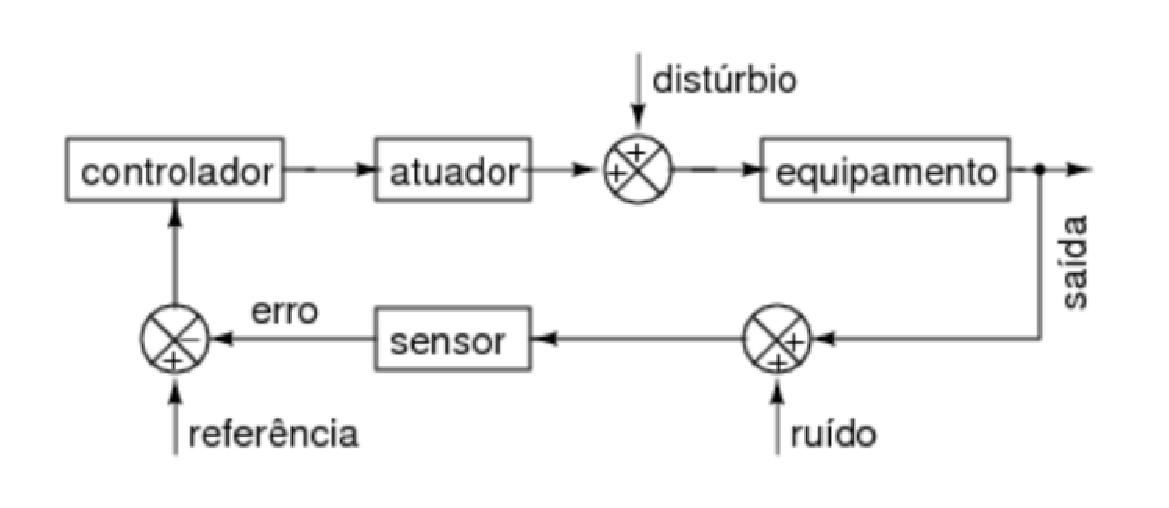
\includegraphics[scale=0.5]{sistema_de_controle}
\caption{Diagrama de Blocos de um Sistema de Controle [5].}
\label{blocoscontrole}
\end{figure}

O sensor é o dispositivo que converte a grandeza física a ser monitorada, no caso do projeto o peso da ração, em um sinal elétrico. Este sinal elétrico é enviado ao microcontrolador para que ele seja comparado com o sinal de referência, que no caso é o peso da ração que deseja-se despejar, caso o valor de ração que se encontra no recipiente dosador ainda esteja abaixo do desejado o sistema continuará a acionar o atuador, que no caso do projeto é o motor CC que controla o fuso que despeja a ração. O fuso continuará despejando ração no recipiente dosador até que o valor desejado seja atingido, quando o sensor medir um valor que ultrapasse o valor desejado o microcontrolador irá verificar e parar o motor do fuso e acionar o motor de passo que abre a comporta do dosador, despejando a ração. Abaixo cada componente deste sistema é explicado mais detalhadamente.

Antes do sistema de alimentação iniciar é necessário verificar se está no horário para a alimentação, caso esteja o procedimento para a alimentação é chamado e o valor da quantidade de ração é passado para a função como mostra o seguinte trecho de código:

\begin{figure}[!h]
\centering 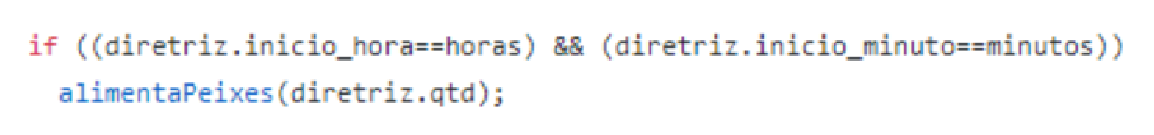
\includegraphics[scale=0.5]{codigo_controle}
\label{codigo_controle1}
 \end{figure}

O seguinte trecho de código mostra como é implementada a comparação entre a variável medida (peso atual de ração no recipiente) e o valor desejado:

\begin{figure}[!h]
\centering 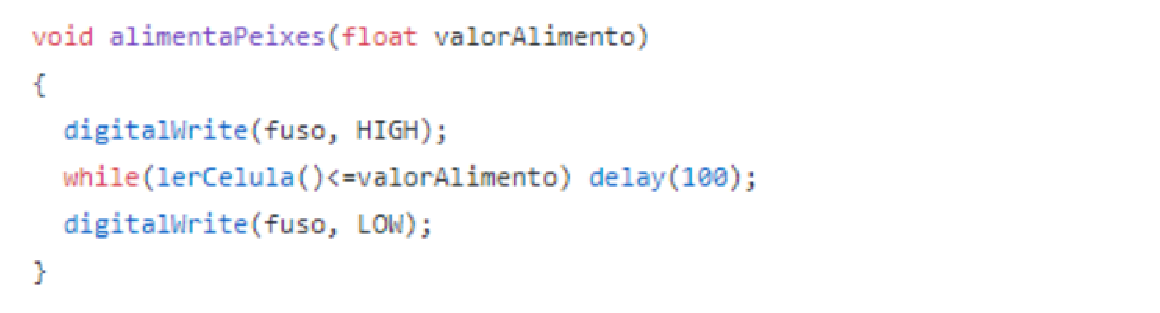
\includegraphics[scale=0.5]{controle2_codigo}
\label{codigo_controle2}
 \end{figure}

O pino que envia o sinal para que o motor do fuso que retira a ração do reservatório e a deposita no dosador é colocado em nível alto, começa-se então o processo de comparação  em um laço while. A função lerCelula() que será explicada mais a frente faz a aquisição dos valores lidos pela célula de carga e realiza a calibração, este valor é comparado com o desejado, quando o ultrapassar o motor é então desligado.

Para a medição do peso de ração recebida pelo dosador escolheu-se utilizar células de carga e um circuito HX711 condicionador de sinais para enviar as medidas para o ATmega. Uma célula de carga é um transdutor que converte uma força feita sobre ele, no caso do projeto, uma carga exercida pela ração, em um sinal elétrico. Este sinal pode ser uma mudança de corrente, uma mudança de tensão ou de frequência dependendo da célula e do circuito em que ela está implementada. As células de carga podem ser de dois tipos: resistiva, que mudam sua resistência quando uma força é aplicada sobre ela, e as capacitivas, que alteram sua capacitância ao ter uma força aplicada sobre ela \cite{loadcell}. A célula de carga utilizada foi do tipo resistiva, ela possui um strain gauge acoplado em sua superfície para medir as variações de compressão.

Um \textit{strain gauge} é um resistor que tem sua resistência variando de acordo com a quantidade de deformação a qual ele é submetido, ele é um dos resistores mais usados para medir peso.  Um strain gauge pode ser visto na figura abaixo:

\begin{figure}[!h]
\centering 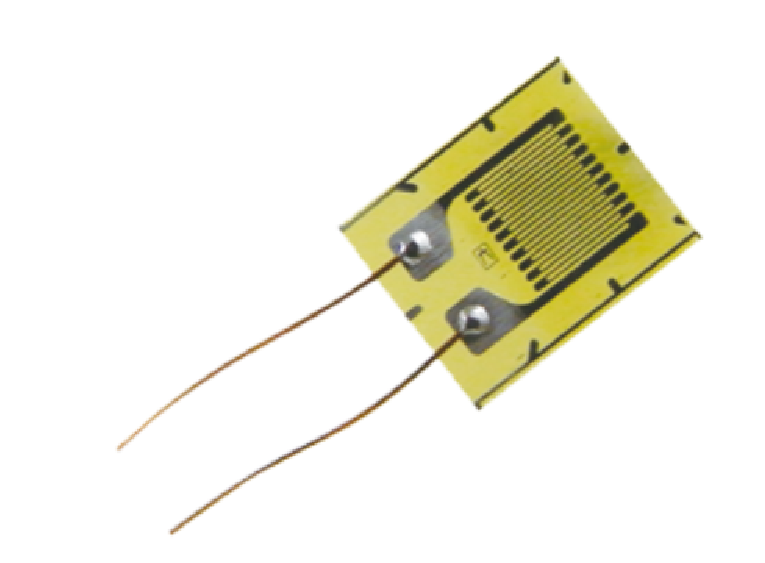
\includegraphics[scale=0.5]{strain_gage}
\caption{Strain Gauge}
\label{straingauge}
 \end{figure}

\pagebreak

A equação \ref{cont1} fornece uma relação entre o fator de gage e a variação de resistência do \textit{strain gauge}.

\begin{equation}
\label{cont1}
\frac{dR}{R}=S \varepsilon
\end{equation}

Onde $R$ é a resistência do material, $\varepsilon$ a deformação do corpo e S o fator de gage, também denominado sensibilidade de deformação \cite{strain}.

Já deformação $\varepsilon$ de um corpo é definida como a razão entre a mudança de comprimento $dl$ de um corpo e o valor quiescente $l$ de comprimento deste corpo, como mostra a equação \ref{cont2}.

\begin{equation}
\label{cont2}
\varepsilon = \frac{dl}{l}
\end{equation}

Um corpo com área de seção transversal uniforme em todo seu comprimento tem sua resistência R definida de acordo com a fórmula \ref{cont3}.

\begin{equation}
\label{cont3}
R=\rho \frac{l}{A}
\end{equation}

Onde $\rho$ é a resistividade do material que compões o \textit{strain gauge}, $l$ o seu comprimento e $A$ a área de sua seção transversal \cite{4785147}.

A figura abaixo apresenta a célula de carga utilizada, ela suporta até 5kg, mas o peso a ser suportado por ela é de, no máximo 10kg, por este motivo foram usadas duas células conectadas em paralelo. O strain gauge presente na superfície da célula de carga forma, em conjunto com três resistores fixos de aproximadamente 1K, uma ponte de Wheatstone para fazer as medições na peso.

\begin{figure}[!h]
\centering 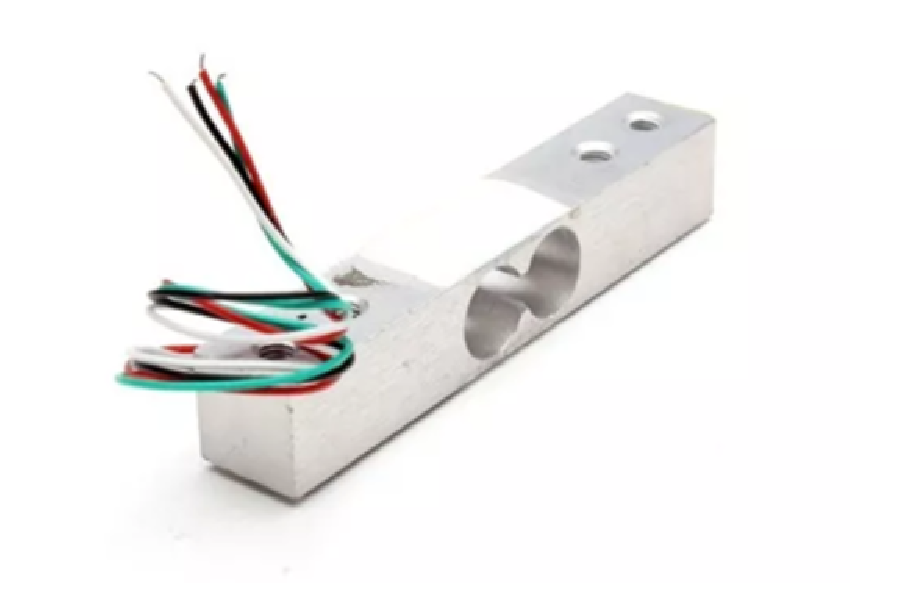
\includegraphics[scale=0.5]{celula_de_carga}
\caption{Célula de carga de 5kg utilizada no projeto.}
\label{celulacarga}
 \end{figure}

A ponte de Wheatstone é usada para traduzir a deformação em uma tensão. Um diagrama de uma ponte de Wheatstone é mostrado na figura abaixo:

\begin{figure}[!h]
\centering 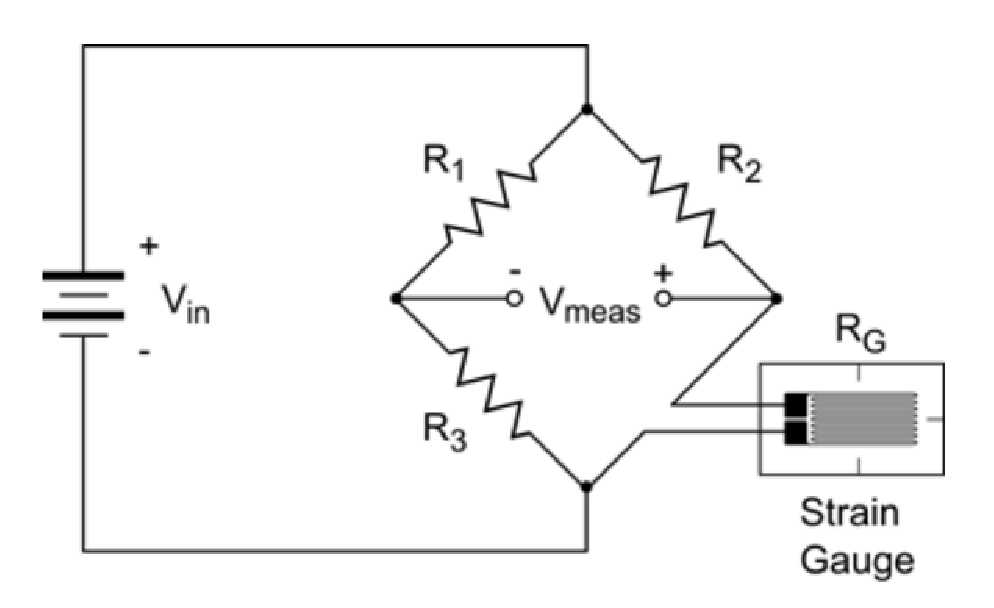
\includegraphics[scale=0.6]{ponte_de_wheatstone}
\caption{ Ponte de Wheatstone encontrada na célula de carga}
\label{wheatstone}
 \end{figure}

A equação \ref{cont4} fornece o valor da tensão $V_{meas}$ em função da deformação do strain gauge, considerando que $R_{1}=R_{2}=R_{3}=R$ e $R_{G}=R+\Delta R$.

\begin{equation}
\label{cont4}
V_{meas}=V_{in} \frac{-\Delta R}{4R+2\Delta R} \approx V_{meas}=V_{in} \frac{-\Delta R}{4R}
\end{equation}

É importante lembrar que o valor de $R=500\Omega$ já que duas pontes estão em paralelo devido ao uso de duas células de carga.

A variação de tensão gerada pela ponte de Wheatstone em resposta à carga colocada sobre as células de carga ainda é baixa e precisa ser amplificada, além disto é necessário que  sinal seja convertido em digital, para isto foi usado o módulo HX711 de 24 bits. Uma ilustração que apresenta um diagrama dos blocos que constituem o módulo é apresentado na figura abaixo:

\begin{figure}[!h]
\centering 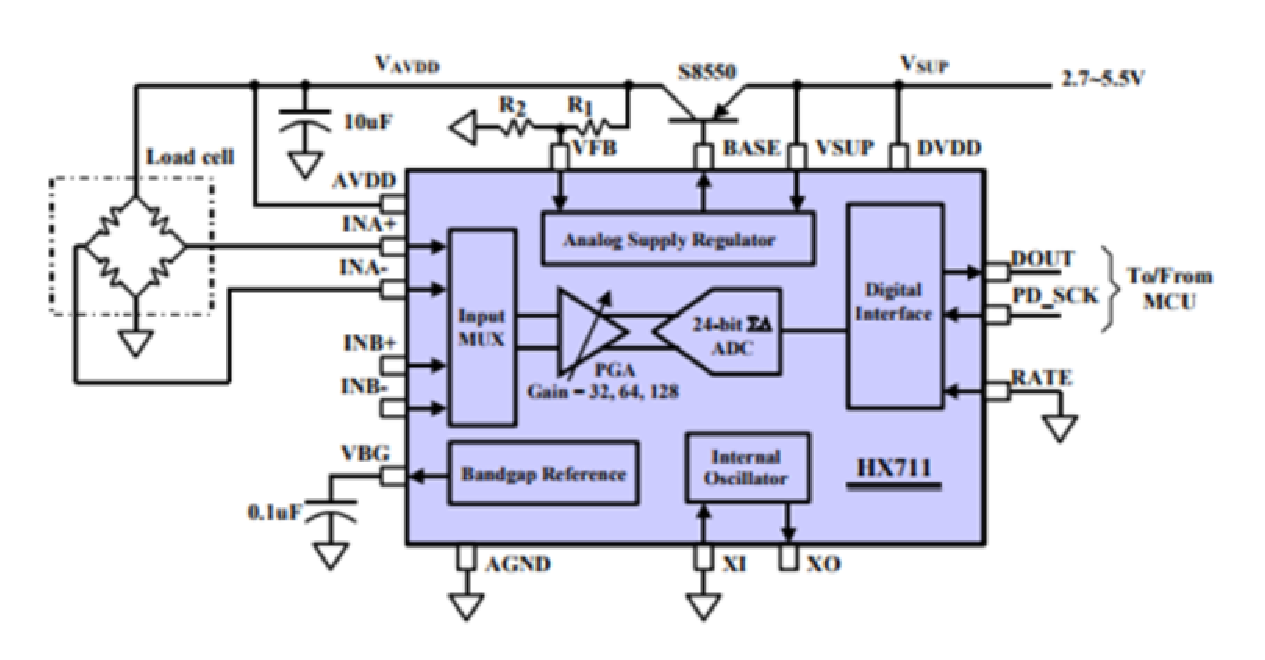
\includegraphics[scale=0.6]{hx711}
\caption{Diagrama de blocos para do módulo Hx711.}
\label{hx711}
 \end{figure}

Ele possui dois canais A e B de entrada para o sinal diferencial que no caso do projeto é o sinal que sai da ponte de Wheatstone, estes canais podem ser selecionados pelo multiplexador interno. Este sinal é amplificado pelo PGA (\textit{Programmable Gain Amplifier}) que pode dar ganho de 64 e 128 para o canal A e 32 para o canal B, o sinal de saída do PGA passa por um conversor AD antes de ser armazenados em seus registradores. Os dados são recuperados dos registradores através dos pinos DOUT e PD\_SCK, o pino DOUT permanece em nível alto até o momento em que a conversão está pronta e os dados podem ser recuperados, neste momento o nível do pino DOUT vai pra baixo. Aplicando 25 pulsos em PD\_SCK os próximos dados obtidos serão do canal A com ganho de 128, 26 pulsos os próximos dados obtidos serão do canal B com ganho de 32 e 27 pulsos os próximos dados obtidos serão do canal A com ganho de 64 \cite{avia:hx711}.

A seguinte função realiza o trabalho de fazer a leitura do módulo, ela é baseada no código fornecido pelo datasheet do circuito e sempre pega o valor que vem do canal A com ganho de 128:

\begin{figure}[!h]
\centering 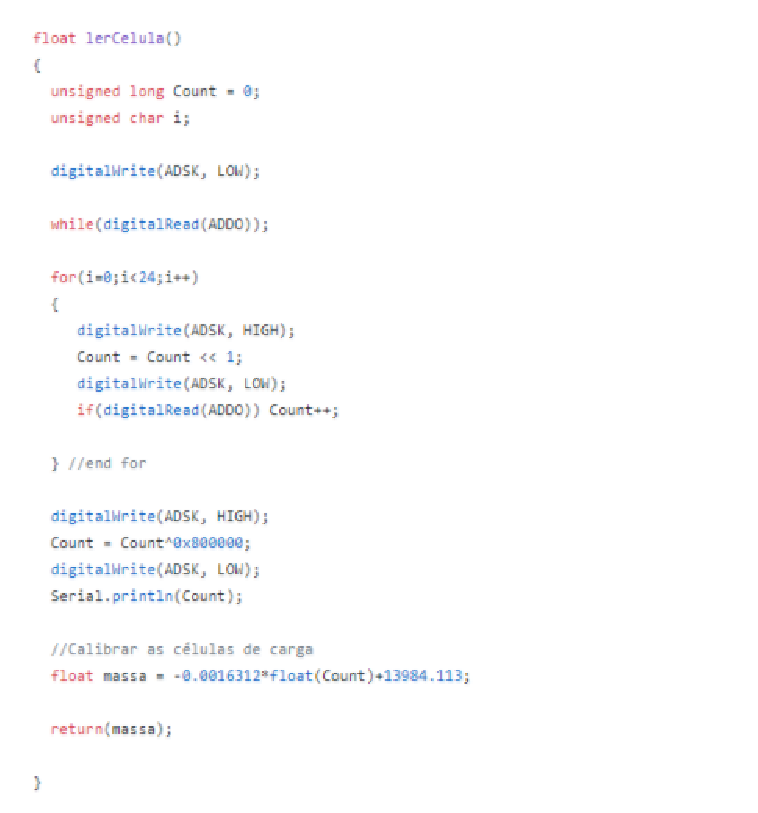
\includegraphics[scale=0.6]{hx711_codigo}

\label{hx711codigo}
 \end{figure}

A função também converte o valor digital de 24 bits vindo do CI para o valor equivalente em massa, para isto foi necessário realizar a calibração das células. O processo de calibração estática consiste em alterar apenas uma variável de entrada e verificar como a saída se comporta com aquela alteração, após o comportamento ser verificado uma função de ajuste que relaciona os valores de saída com os de entrada é traçada. A resultado obtido é apresentado no gráfico abaixo:

\begin{figure}[!h]
\centering 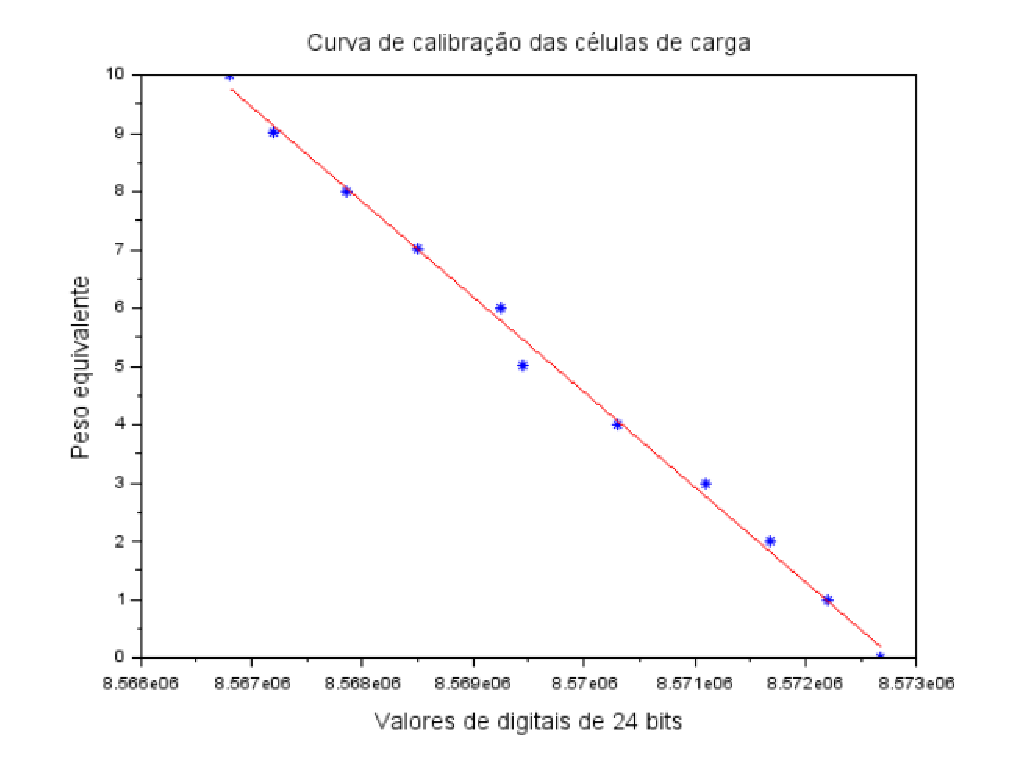
\includegraphics[scale=0.6]{calibracao_celula_de_carga}
\label{calibracaocelula}
 \end{figure}

\pagebreak

A curva obtida foi colocada dentro da função lerCelula() para fazer a conversão.

Para ligar e desligar o motor do fuso escolheu-se utilizar o relé HJR1-2C que será acionado pelo transistor TBJ BC548. o relé suporta até 2A o que é suficiente já que a corrente do motor é de 1,58A.

\subsection{Sensores Secundários}

A temperatura externa ao tanque será adquirida pelo sensor digital Ds18b20, que possui uma faixa dinâmica de medição de -10°C a +85°C. O sinal é totalmente transmitido de forma digital para o microcontrolador via protocolo OneWire.

\begin{figure}[!h]
\centering 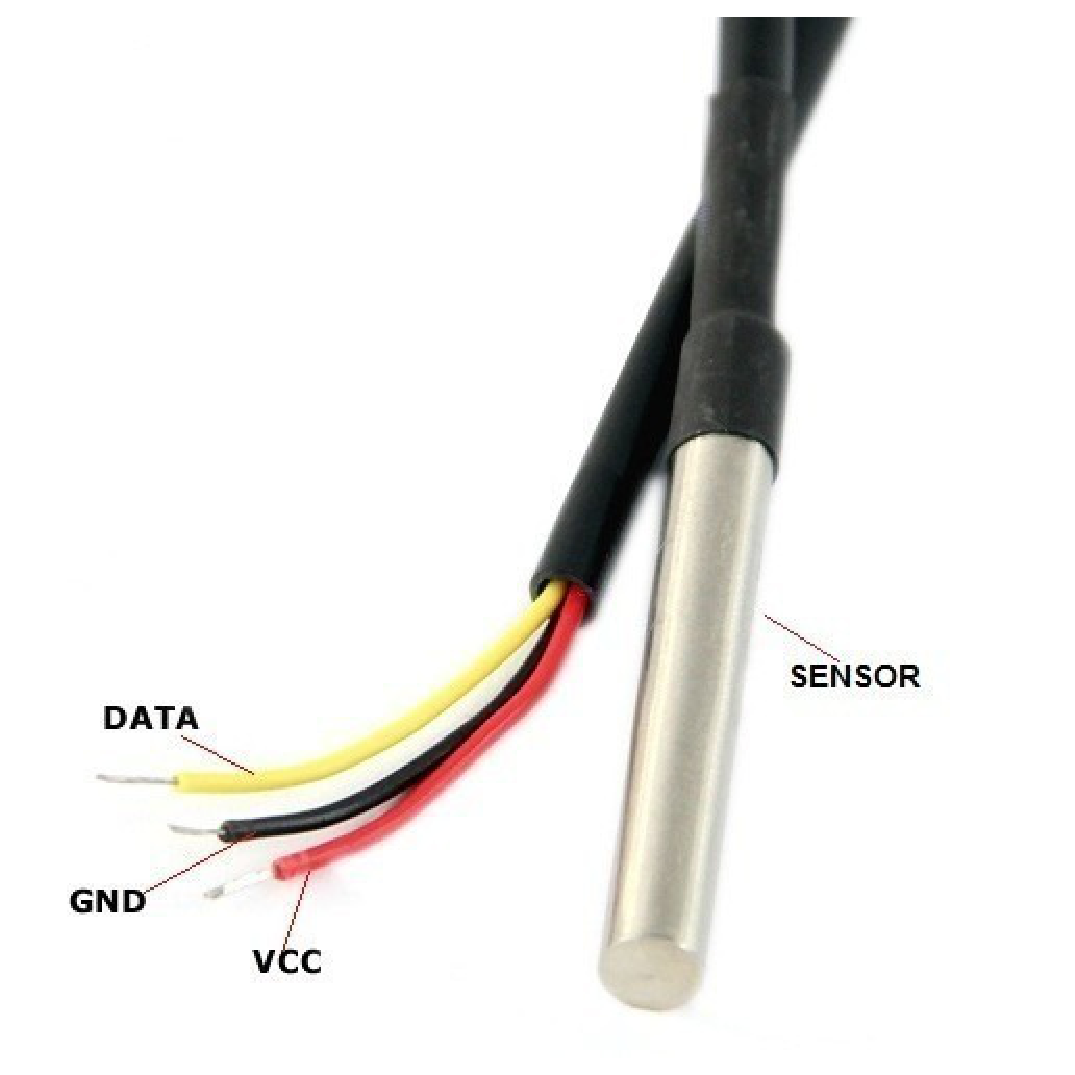
\includegraphics[scale=0.5]{sensor_temperatura}
\caption{Sensor de temperatura Ds18b20 e a função de cada pino.}
\label{sensortemp}
\end{figure}


\pagebreak

O sensor já se encontra pré-calibrado de fábrica e envia o valor de temperatura já convertido.
Para obter corretamente os dados do sensor dentro do programa, é necessário utilizar a biblioteca fornecida pelo fabricante e configurar o pino do microcontrolador para funcionar como barramento OneWire. Depois é necessário instanciar objeto responsável pelo sensor dentro do código, onde periodicamente é chamado o método responsável por receber os valores já convertidos. \cite{avia:temp}

Para medir a condutividade da água, optou-se por confeccionar um sensor próprio. Ele é baseado em medir o quanto que um sinal triangular é atenuado entre eletrodos submersos na água, de acordo com \cite{avia:condut}.

\begin{figure}[!h]
\centering 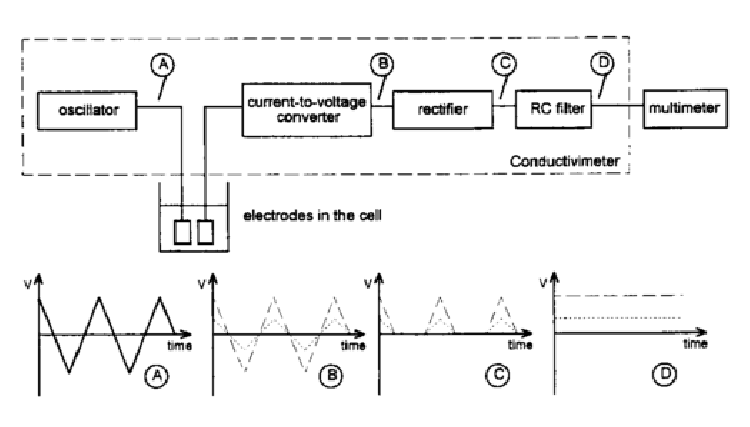
\includegraphics[scale=0.5]{condutivimetro}
\caption{Estágios conceituais do condutivímetro a ser confeccionado.}
\label{estagcondu}
\end{figure}

O sensor funciona através de quatro estágios de circuitos, em que o primeiro é um oscilador triangular que gera uma corrente no eletrodo, onde essa corrente é capatada por um conversor de corrente-para-tensão, onde o sinal resultante é retificado e depois filtrado por um filtro passivo RC. O saída resultante é um sinal contínuo com valores entre 0V a 5V (amplitude da onda triangular gerada).


\subsection{Projeto da PCB}

Método utilizado para a confecção da placa foi o fotográfico pois é o de melhor qualidade e riqueza de detalhes, este processo é constituído de 12 etapas:

1. Esquema elétrico e circuito eletrônico – Nessa etapa foi utilizado um software livre (Fritzing) para a criação do circuito tanto na protoboard quanto o circuito elétrico.


2. Layout do circuito impresso a partir do esquema elétrico -  O software Fritzing novamente foi utilizado gerando um fotolito que permitiu uma economia de matérias como percloreto de ferro e o tamanho das placas de fenolite.

3. Impressão do fotolito -  Foi utilizado uma impressora laser e um fotolito compatível com a impressora.

4. Sincronismo das faces - O alinhamento ocorreu apenas na camada existente

5. Limpeza da placa - A placa foi limpa com detergente e esponja vegetal

6. Aplicação do Dryfilm ou tinta fotossensível -  Neste caso foi utilizado a tinta foto sensível pois apesar de não ter uma qualidade tão elevada quanto o Dryfilm apresenta um custo menor

7. Alinhamento dos fotolitos e Fotografia - O alinhamento ocorreu apenas na camada existente

8. Revelação – Foi utilizada luz ultra violeta de 27w por 4 minutos a uma distância de 20 cm da placa

9. Corrosão – com percloreto de ferro

10. Remoção do dryfilm residual – A placa foi mergulhada em 250ml de uma solução de 10\% de hidróxido de sódio.

11. Furos para os componentes – A placa foi perfurada com uma broca de 1mm de diâmetro.

12. Aplicar Verniz nas placas de PCI – Esta etapa não foi efetuada pois ainda esta na etapa de testes


\begin{figure}[!h]
\centering \includegraphics[scale=0.13]{pcb4}
\caption{fotolito.}
\label{sensortemp}
\end{figure}


\begin{figure}[!h]
\centering \includegraphics[scale=0.14]{pcb1}
\caption{Placa na etapa 10.}
\label{sensortemp}
\end{figure}



\begin{figure}[!h]
\centering \includegraphics[scale=0.16]{detalhe-placa}
\caption{Detalhamento da placa na etapa 10.}
\label{sensortemp}
\end{figure}



\begin{figure}[!h]
\centering \includegraphics[scale=0.16]{pcb3}
\caption{Placa após o término.}
\label{sensortemp}
\end{figure}
